\documentclass[journal,12pt,twocolumn]{IEEEtran}
\usepackage{setspace}
\usepackage{gensymb}
\usepackage{caption}
%\usepackage{multirow}
%\usepackage{multicolumn}
%\usepackage{subcaption}
%\doublespacing
\singlespacing
\usepackage{csvsimple}
\usepackage{amsmath}
\usepackage{multicol}
%\usepackage{enumerate}
\usepackage{amssymb}
%\usepackage{graphicx}
\usepackage{newfloat}
%\usepackage{syntax}
\usepackage{listings}
\usepackage{iithtlc}
\usepackage{color}
\usepackage{tikz}
\usetikzlibrary{shapes,arrows}



%\usepackage{graphicx}
%\usepackage{amssymb}
%\usepackage{relsize}
%\usepackage[cmex10]{amsmath}
%\usepackage{mathtools}
%\usepackage{amsthm}
%\interdisplaylinepenalty=2500
%\savesymbol{iint}
%\usepackage{txfonts}
%\restoresymbol{TXF}{iint}
%\usepackage{wasysym}
\usepackage{amsthm}
\usepackage{mathrsfs}
\usepackage{txfonts}
\usepackage{stfloats}
\usepackage{cite}
\usepackage{cases}
\usepackage{mathtools}
\usepackage{caption}
\usepackage{enumerate}	
\usepackage{enumitem}
\usepackage{amsmath}
%\usepackage{xtab}
\usepackage{longtable}
\usepackage{multirow}
%\usepackage{algorithm}
%\usepackage{algpseudocode}
\usepackage{enumitem}
\usepackage{mathtools}
\usepackage{hyperref}
%\usepackage[framemethod=tikz]{mdframed}
\usepackage{listings}
    %\usepackage[latin1]{inputenc}                                 %%
    \usepackage{color}                                            %%
    \usepackage{array}                                            %%
    \usepackage{longtable}                                        %%
    \usepackage{calc}                                             %%
    \usepackage{multirow}                                         %%
    \usepackage{hhline}                                           %%
    \usepackage{ifthen}                                           %%
  %optionally (for landscape tables embedded in another document): %%
    \usepackage{lscape}     


\usepackage{url}
\def\UrlBreaks{\do\/\do-}


%\usepackage{stmaryrd}


%\usepackage{wasysym}
%\newcounter{MYtempeqncnt}
\DeclareMathOperator*{\Res}{Res}
%\renewcommand{\baselinestretch}{2}
\renewcommand\thesection{\arabic{section}}
\renewcommand\thesubsection{\thesection.\arabic{subsection}}
\renewcommand\thesubsubsection{\thesubsection.\arabic{subsubsection}}

\renewcommand\thesectiondis{\arabic{section}}
\renewcommand\thesubsectiondis{\thesectiondis.\arabic{subsection}}
\renewcommand\thesubsubsectiondis{\thesubsectiondis.\arabic{subsubsection}}

% correct bad hyphenation here
\hyphenation{op-tical net-works semi-conduc-tor}

%\lstset{
%language=C,
%frame=single, 
%breaklines=true
%}

%\lstset{
	%%basicstyle=\small\ttfamily\bfseries,
	%%numberstyle=\small\ttfamily,
	%language=Octave,
	%backgroundcolor=\color{white},
	%%frame=single,
	%%keywordstyle=\bfseries,
	%%breaklines=true,
	%%showstringspaces=false,
	%%xleftmargin=-10mm,
	%%aboveskip=-1mm,
	%%belowskip=0mm
%}

%\surroundwithmdframed[width=\columnwidth]{lstlisting}
\def\inputGnumericTable{}                                 %%
\lstset{
%language=C,
frame=single, 
breaklines=true,
columns=fullflexible
}
 

\begin{document}
%
\tikzstyle{block} = [rectangle, draw,
    text width=3em, text centered, minimum height=3em]
\tikzstyle{sum} = [draw, circle, node distance=3cm]
\tikzstyle{input} = [coordinate]
\tikzstyle{output} = [coordinate]
\tikzstyle{pinstyle} = [pin edge={to-,thin,black}]

\theoremstyle{definition}
\newtheorem{theorem}{Theorem}[section]
\newtheorem{problem}{Problem}
\newtheorem{proposition}{Proposition}[section]
\newtheorem{lemma}{Lemma}[section]
\newtheorem{corollary}[theorem]{Corollary}
\newtheorem{example}{Example}[section]
\newtheorem{definition}{Definition}[section]
%\newtheorem{algorithm}{Algorithm}[section]
%\newtheorem{cor}{Corollary}
\newcommand{\BEQA}{\begin{eqnarray}}
\newcommand{\EEQA}{\end{eqnarray}}
\newcommand{\define}{\stackrel{\triangle}{=}}

\bibliographystyle{IEEEtran}
%\bibliographystyle{ieeetr}

\providecommand{\nCr}[2]{\,^{#1}C_{#2}} % nCr
\providecommand{\nPr}[2]{\,^{#1}P_{#2}} % nPr
\providecommand{\mbf}{\mathbf}
\providecommand{\pr}[1]{\ensuremath{\Pr\left(#1\right)}}
\providecommand{\qfunc}[1]{\ensuremath{Q\left(#1\right)}}
\providecommand{\sbrak}[1]{\ensuremath{{}\left[#1\right]}}
\providecommand{\lsbrak}[1]{\ensuremath{{}\left[#1\right.}}
\providecommand{\rsbrak}[1]{\ensuremath{{}\left.#1\right]}}
\providecommand{\brak}[1]{\ensuremath{\left(#1\right)}}
\providecommand{\lbrak}[1]{\ensuremath{\left(#1\right.}}
\providecommand{\rbrak}[1]{\ensuremath{\left.#1\right)}}
\providecommand{\cbrak}[1]{\ensuremath{\left\{#1\right\}}}
\providecommand{\lcbrak}[1]{\ensuremath{\left\{#1\right.}}
\providecommand{\rcbrak}[1]{\ensuremath{\left.#1\right\}}}
\theoremstyle{remark}
\newtheorem{rem}{Remark}
\newcommand{\sgn}{\mathop{\mathrm{sgn}}}
\providecommand{\abs}[1]{\left\vert#1\right\vert}
\providecommand{\res}[1]{\Res\displaylimits_{#1}} 
\providecommand{\norm}[1]{\lVert#1\rVert}
\providecommand{\mtx}[1]{\mathbf{#1}}
\providecommand{\mean}[1]{E\left[ #1 \right]}
\providecommand{\fourier}{\overset{\mathcal{F}}{ \rightleftharpoons}}
%\providecommand{\hilbert}{\overset{\mathcal{H}}{ \rightleftharpoons}}
\providecommand{\system}{\overset{\mathcal{H}}{ \longleftrightarrow}}
	%\newcommand{\solution}[2]{\textbf{Solution:}{#1}}
\newcommand{\solution}{\noindent \textbf{Solution: }}
\newcommand{\myvec}[1]{\ensuremath{\begin{pmatrix}#1\end{pmatrix}}}
\providecommand{\dec}[2]{\ensuremath{\overset{#1}{\underset{#2}{\gtrless}}}}
\DeclarePairedDelimiter{\ceil}{\lceil}{\rceil}
%\numberwithin{equation}{subsection}
\numberwithin{equation}{section}
%\numberwithin{problem}{subsection}
%\numberwithin{definition}{subsection}
\makeatletter
\@addtoreset{figure}{section}
\makeatother

\let\StandardTheFigure\thefigure
%\renewcommand{\thefigure}{\theproblem.\arabic{figure}}
\renewcommand{\thefigure}{\thesection}


%\numberwithin{figure}{subsection}

%\numberwithin{equation}{subsection}
%\numberwithin{equation}{section}
%\numberwithin{equation}{problem}
%\numberwithin{problem}{subsection}
\numberwithin{problem}{section}
%%\numberwithin{definition}{subsection}
%\makeatletter
%\@addtoreset{figure}{problem}
%\makeatother
\makeatletter
\@addtoreset{table}{section}
\makeatother

\let\StandardTheFigure\thefigure
\let\StandardTheTable\thetable
\let\vec\mathbf
%%\renewcommand{\thefigure}{\theproblem.\arabic{figure}}
%\renewcommand{\thefigure}{\theproblem}

%%\numberwithin{figure}{section}

%%\numberwithin{figure}{subsection}



\def\putbox#1#2#3{\makebox[0in][l]{\makebox[#1][l]{}\raisebox{\baselineskip}[0in][0in]{\raisebox{#2}[0in][0in]{#3}}}}
     \def\rightbox#1{\makebox[0in][r]{#1}}
     \def\centbox#1{\makebox[0in]{#1}}
     \def\topbox#1{\raisebox{-\baselineskip}[0in][0in]{#1}}
     \def\midbox#1{\raisebox{-0.5\baselineskip}[0in][0in]{#1}}

\vspace{3cm}

\title{ 
	\logo{
Linear Algebra through Coordinate Geometry 
	}
}

\author{ G V V Sharma$^{*}$% <-this % stops a space
	\thanks{*The author is with the Department
		of Electrical Engineering, Indian Institute of Technology, Hyderabad
		502285 India e-mail:  gadepall@iith.ac.in. All content in this manual is released under GNU GPL.  Free and open source.}
	
}	

\maketitle

\tableofcontents

\bigskip

\renewcommand{\thefigure}{\theenumi}
\renewcommand{\thetable}{\theenumi}


\begin{abstract}
	
This manual introduces linear algebra through coordinate geometry using a problem solving approach.
\end{abstract}
|\section{The Straight Line}
\begin{enumerate}[label=\thesection.\arabic*
,ref=\thesection.\theenumi]
\item The equation of the line between two points $\vec{A}$ and $\vec{B}$ is given by
\begin{equation}
\vec{x} = \vec{A} + \lambda \brak{\vec{A}-\vec{B}}
\end{equation}
%
Alternatively, it can be expressed as
\begin{equation}
\label{eq:line_normal}
\vec{n}^T\brak{\vec{x}-\vec{A}} = 0
\end{equation}
%
where $\vec{n}$ is the solution of
\begin{equation}
\label{eq:normal_slope}
\brak{\vec{A}-\vec{B}}^T\vec{n} = 0
\end{equation}
\item In $\triangle ABC$,
\begin{equation}
\label{eq:linea}
\vec{A}=\myvec{1\\2}
\end{equation}
%
and the equations of the medians through $\vec{B}$ and $\vec{C}$
are respectively
\begin{align}
\label{eq:line_medb}
\myvec{1 & 1}\vec{x}&=5
\\
\myvec{1 & 0}\vec{x}&=4
\label{eq:line_medc}
\end{align}
%
Find the area of $\triangle ABC$.
\\
\solution The centroid $\vec{O}$ is the solution of \eqref{eq:line_medb},\eqref{eq:line_medc} and is obtained 
as the solution
of the matrix equation
\begin{align}
\myvec{1 & 1 \\1 & 0}\vec{x}&=\myvec{5 \\ 4}
\label{eq:line_matrix}
\end{align}
%
which can be solved using the augmented matrix as follows.
\begin{align}
\myvec{1 & 1 & 5\\1 & 0 & 4} \leftrightarrow \myvec{1 & 1 & 5\\0 & 1 & 1}\leftrightarrow  \myvec{1 & 0 & 4\\0 & 
1 & 1}
\end{align}
Thus,
\begin{equation}
\label{eq:lineo}
\vec{O}=\myvec{4\\1}
\end{equation}
% 
Let  $AD$ be the median through $\vec{A}$. Then,
\begin{align}
\frac{\vec{A}+\vec{B}+\vec{C}}{3}&= \vec{O}
\\
\implies \vec{B}+\vec{C}= 3\vec{O}-\vec{A} &= \myvec{11 \\ 1}
\label{eq:line_b+c}
\\
\implies \myvec{1 & 1}\vec{B}+\myvec{1 & 1}\vec{C}&=  \myvec{1 & 1}\myvec{11 \\ 1}
\label{eq:line_ctemp}
\end{align}
%
From \eqref{eq:line_medc} and \eqref{eq:line_ctemp},
\begin{align}
 \myvec{1 & 1}\vec{B} &= 5 
\\
\implies 5+\myvec{1 & 1}\vec{C}&=  12
\\
\implies \myvec{1 & 1}\vec{C}&=  7
\label{eq:line_ctemp2}
\end{align}
From \eqref{eq:line_ctemp2} and \eqref{eq:line_medc}, $\vec{C}$ can be obtained by solving 
\begin{align}
\myvec{1 & 1 \\1 & 0}\vec{C}&=\myvec{7 \\ 4}
\label{eq:line_cmatrix}
\end{align}
using the augmented matrix as
\begin{align}
\myvec{1 & 1 & 7\\1 & 0 & 4} &\leftrightarrow \myvec{1 & 1 & 7\\0 & 1 & 3}\leftrightarrow \myvec{1 & 0 & 4\\0 & 
1 & 3}
\\
\implies \vec{C}&=\myvec{4\\3}
\end{align}
%
From \eqref{eq:line_b+c},
\begin{align}
\vec{B}&=\myvec{11\\1}-\myvec{4\\3}
=\myvec{7\\-2}
\end{align}
%
Thus,
\begin{align}
\frac{1}{2}
\begin{vmatrix}
\vec{A} & \vec{B} &\vec{C}
\\
1 & 1 & 1
\end{vmatrix}
=
\frac{1}{2}
\begin{vmatrix}
1 & 7 & 4\\2 & -2 & 3 \\ 1 & 1 & 1
\end{vmatrix} = 9
\end{align}
\end{enumerate}
\section{Orthogonality}
\begin{enumerate}[label=\thesection.\arabic*
,ref=\thesection.\theenumi]
\item $\vec{u}^T\vec{x} = 0 \implies \vec{u} \perp \vec{x}$. Show that 
\begin{align}
\label{eq:orth_parallel}
\vec{u}^T\vec{x}  = \vec{P}^T\vec{x} = 0 \implies \vec{P} =\alpha 
\vec{u}
\end{align}
%
\item The foot of the perpendicular drawn from the origin on the line 
\begin{align}
\label{eq:orth_line}
AB: \vec{u}^T\vec{x}  =\lambda
\end{align}
where
\begin{align}
\vec{u}=\myvec{3 \\ 1}
\end{align}
is $\vec{P}$.  The line meets the $x$-axis at $\vec{A}$ and $y$-axis at $\vec{B}$. Show that $\vec{P} =\alpha 
\vec{u}$ and find $\alpha$.
\\
\solution From \eqref{eq:orth_line},
\begin{align}
\vec{u}^T\vec{A}=\vec{u}^T\vec{B}=\lambda
\\
\implies \vec{u}^T\brak{\vec{A}-\vec{B}}=0
\end{align}
%
Since $OP \perp AB$,
\begin{align}
\vec{P}^T\brak{\vec{A}-\vec{B}}=0
\end{align}
%
Thus, from \eqref{eq:orth_parallel},
\begin{align}
\vec{P} =\alpha \vec{u}
\label{eq:orth_purel}
\end{align}
%
Since $\vec{P} $ lies on \eqref{eq:orth_line},
\begin{align}
\vec{u}^T\vec{P}=\alpha\vec{u}^T\vec{u}=\lambda
\\
\implies \alpha = \frac{\lambda}{\vec{u}^T\vec{u}} = \frac{\lambda}{10}.
\label{eq:orth_alpha}
\end{align}
%
\item Find $\vec{A} $.
\\
\solution Let
\begin{equation}
\vec{A} = a\myvec{1 \\ 0}
\label{eq:orth_adef}
\end{equation}
From \eqref{eq:orth_line},
\begin{align}
\vec{u}^T\vec{A} &= a\myvec{3 & 1}\myvec{1 \\ 0} = \lambda
\\
\implies a &= \frac{\lambda}{3}
\label{eq:orth_a}
\\
\text{and } \vec{A} &= \frac{\lambda}{3}\myvec{1 \\ 0}
\end{align}

\item Find the ratio $BP:PA$.
\\
\solution Let
\begin{align}
\frac{BP}{PA}= k
\end{align}
%
Then, 
\begin{align}
k\vec{A} + \vec{B} &= \brak{k+1}\vec{P}
\\
\implies k\vec{A}^T\vec{A} + \vec{A}^T\vec{B} &= \brak{k+1}\vec{P}^T\vec{A}
\\
\implies ka^2  &= \alpha\brak{k+1}\lambda
\end{align}
%
using \eqref{eq:orth_purel},  \eqref{eq:orth_adef}, \eqref{eq:orth_line} and $\vec{A}\perp \vec{B}$. 
Substituting from \eqref{eq:orth_alpha} and 
\eqref{eq:orth_a},
\begin{align}
\implies k\frac{\lambda^2}{9}  &= \brak{k+1}\frac{\lambda^2}{10}
\\
\implies k  &= 9
\end{align}

\end{enumerate}

\section{Locus}
\begin{enumerate}[label=\thesection.\arabic*
,ref=\thesection.\theenumi]
\item The line through
\begin{equation}
\label{eq:locus}
\vec{A}=\myvec{2\\3}
\end{equation}
intersects the coordinate axes at $\vec{P}$ and $\vec{Q}$.  $\vec{O}$ is the origin and rectangle $OPRQ$ is 
completed as shown in Fig. \eqref{fig:locus},
\begin{figure}
\centering
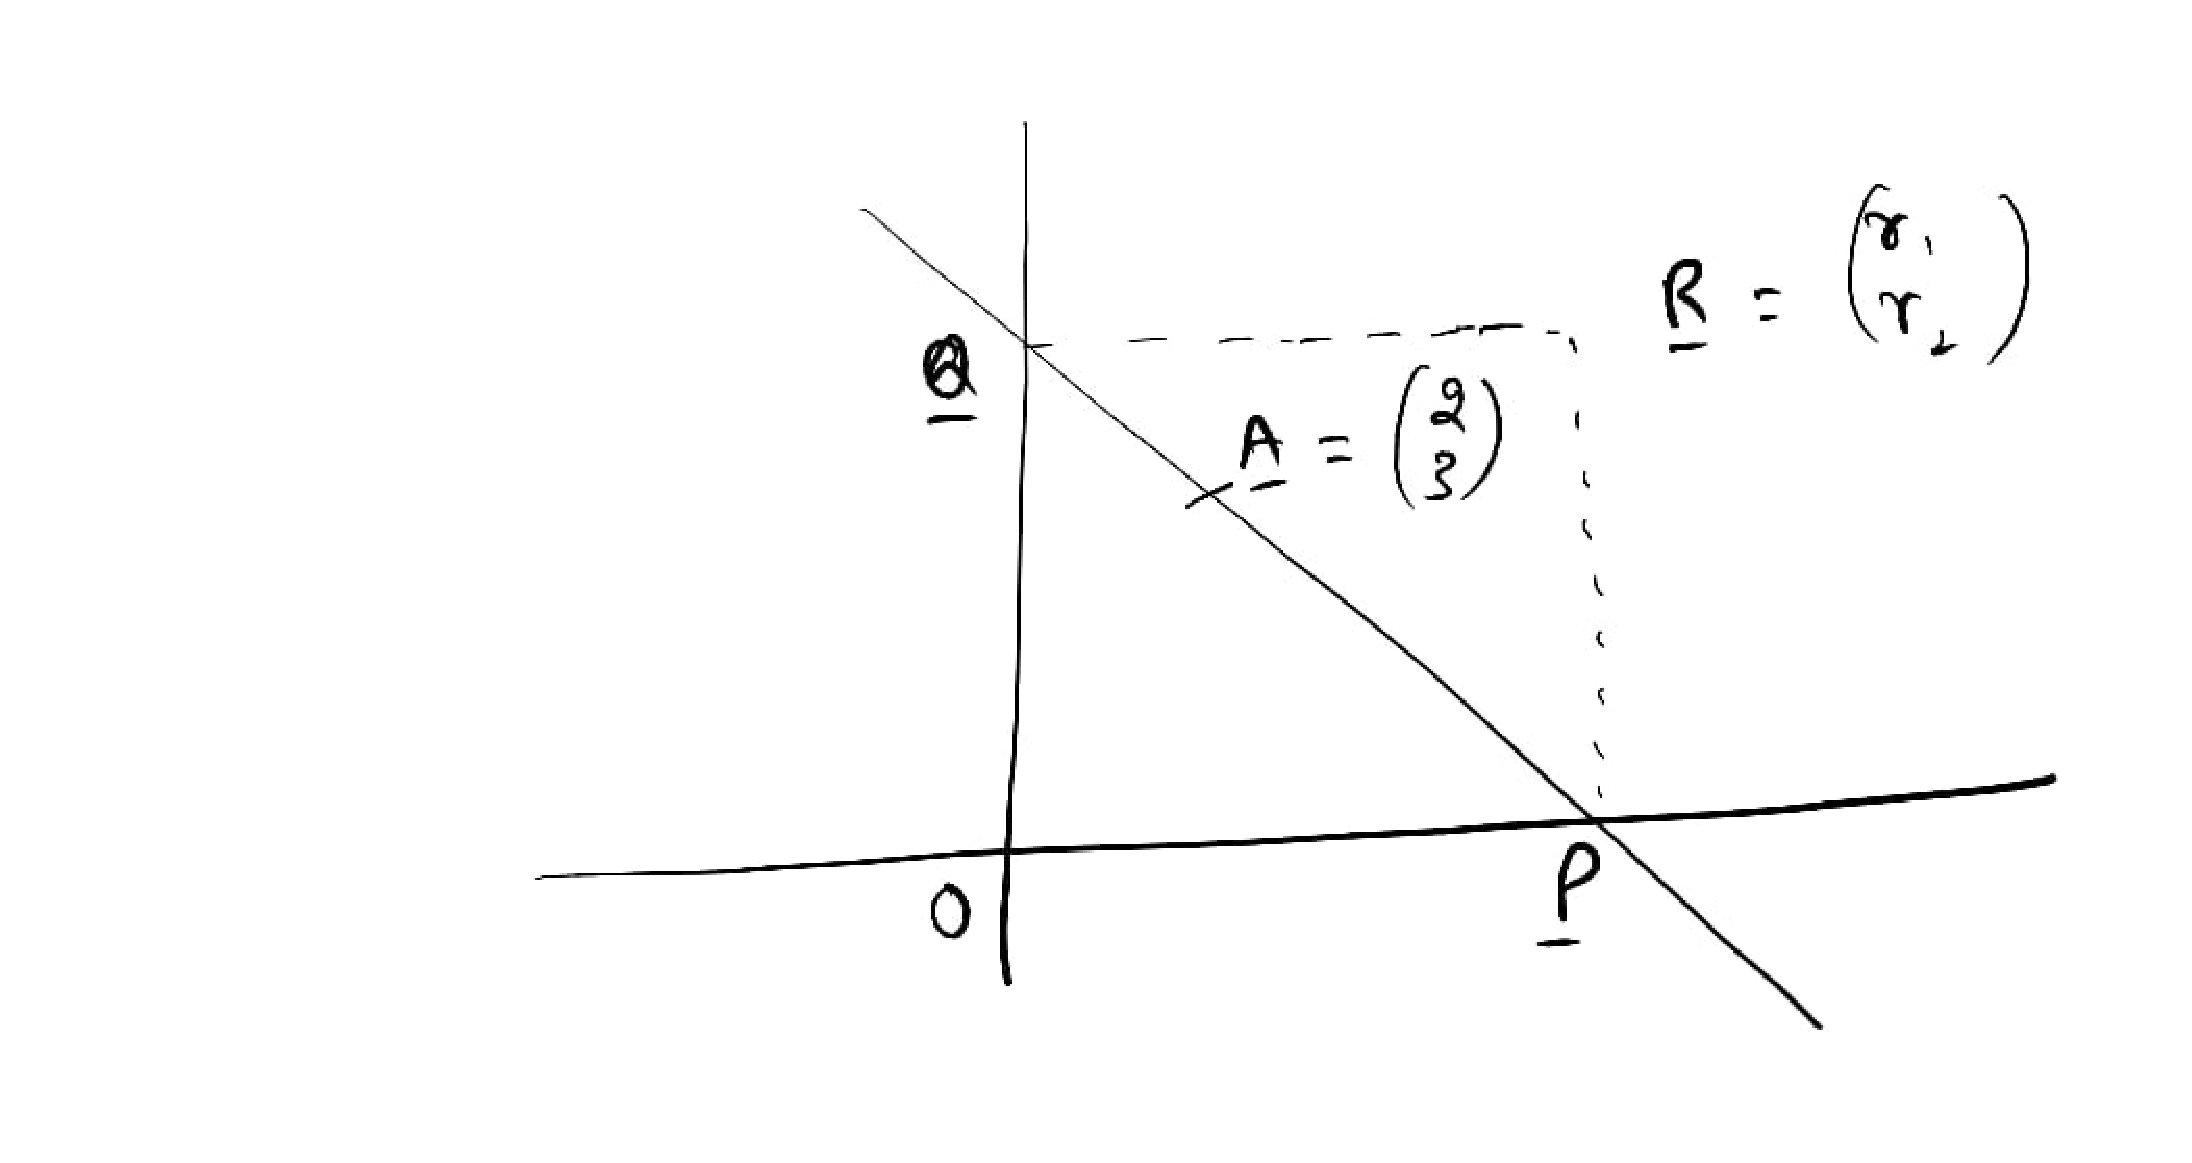
\includegraphics[width=\columnwidth]{./figs/locus.eps}
\caption{}
\label{fig:locus}
\end{figure}
\item Show that
\begin{align}
\vec{P}&= \myvec{1 & 0\\ 0 & 0}\vec{R}
\label{eq:locusp}
\\
\vec{Q}&= \myvec{0 & 0\\ 0 & 1}\vec{R}
\label{eq:locusq}
\\
\vec{P}+\vec{Q} &=\vec{R}
\label{eq:locusr}
\end{align}
\item Show that
\begin{align}
\begin{split}
\brak{\vec{A}-\vec{P}}^T\vec{n} &= 0
\\
\brak{\vec{A}-\vec{Q}}^T\vec{n} &= 0
\\
\brak{\vec{P}-\vec{Q}}^T\vec{n} &= 0
\end{split}
\label{eq:locus_apq}
\end{align}
\\
\solution 
Trivial using \eqref{eq:line_normal} and \eqref{eq:normal_slope}.
%
\item Show that
\begin{align}
\brak{2\vec{A}-\vec{R}}^T\vec{n} &= 0
\label{eq:locusm1}
\\
\label{eq:locusm2}
\vec{R}^T\myvec{1 & 0\\ 0 & -1}\vec{n} &= 0
\end{align}
\\
\solution
From \eqref{eq:locus_apq} and \eqref{eq:locusr}
\begin{align}
\sbrak{2\vec{A}-\brak{\vec{P}+\vec{Q}}}^T\vec{n} = 0
\end{align}
%
resulting in  \eqref{eq:locusm1}.
From \eqref{eq:locus_apq} and \eqref{eq:locusp},\eqref{eq:locusq}, \eqref{eq:locusm2} is obtained.
%
\item Show that
\begin{equation}
\vec{R}^{T}\myvec{0 & -1\\ 1 & 0}\vec{R} = 0.
\end{equation}
\item Find the locus of $\vec{R}$.
\\
\solution
For $\vec{n}$ to be unique in \eqref{eq:locusm1},\eqref{eq:locusm2},
\begin{multline}
\brak{2\vec{A}-\vec{R}} = k \myvec{1 & 0\\ 0 & -1}\vec{R}
\\
\implies \vec{R}^{T}\myvec{0 & 1\\ 1 & 0}\brak{\vec{2A}-\vec{R}} 
\\
= k \vec{R}^{T}\myvec{0 & 1\\ 1 & 0}\myvec{1 & 0\\ 0 & -1}\vec{R}
\\
= k \vec{R}^{T}\myvec{0 & -1\\ 1 & 0}\vec{R} = 0
\end{multline}
%
where $k$ is some constant.  Thus, the desired locus is
\begin{align}
 \vec{R}^{T}\myvec{0 & 1\\ 1 & 0}\brak{2\vec{A}-\vec{R}} 
&= 0
\\
\implies \vec{R}^{T}\myvec{0 & 1\\ 1 & 0}\vec{R}- 2\vec{A}^T\vec{R}
&= 0
\end{align}
\end{enumerate}
%
\section{Conics}
\begin{enumerate}[label=\thesection.\arabic*
,ref=\thesection.\theenumi]
\item The equation of a quadratic curve is given by
\begin{equation}
Ax_1^2+Bx_1x_2+Cx_2^2+Dx_1+Ex_2+F = 0
\label{eq:quadratic}
\end{equation}
%
Show that  \eqref{eq:quadratic} can be expressed as
\begin{equation}
\vec{x}^TV\vec{x}+2\vec{u}^T\vec{x}+ F = 0
\label{eq:quadratic_vec}
\end{equation}
%
Find the matrix $V$ and vector $\vec{u}$.
\item The tangent to \eqref{eq:quadratic} at a point $\vec{p}$ on the curve is given by
\begin{equation}
\myvec{\vec{p}^T & 1}\myvec{V & \vec{u} \\ \vec{u}^T & F} \myvec{\vec{x} \\ 1} = 0
\label{eq:tangent_one}
\end{equation}
%
Show that \eqref{eq:tangent_one} can be expressed as
\begin{equation}
\brak{\vec{p}^TV+\vec{u}^T}\vec{x} + \vec{p}^T\vec{u} +F = 0
\label{eq:tangent}
\end{equation}
\item Classify the various conic sections based on $\eqref{eq:quadratic_vec}$.
\\
\solution 
\begin{table}[!hb]
\centering
\input{./figs/conics.tex}
\caption{}
\label{table:conics}
\end{table}

\end{enumerate}
\section{Circle}
\begin{enumerate}[label=\thesection.\arabic*
,ref=\thesection.\theenumi]
\item Find the tangent to the circle
\begin{equation}
C_1: \vec{x}^T\vec{x} - \myvec{2 & 0}\vec{x} 
-1 = 0 
\end{equation}
%
at the point $\myvec{2 \\1}$.
\\
\solution From \eqref{eq:tangent_one}, the tangent $T$ is given by
\begin{align}
\sbrak{\myvec{2 & 1}-\myvec{1 & 0}}\vec{x} -\myvec{2 & 1}\myvec{1 \\ 0}  &= 1
\\
\implies T: \vec{n}^T\vec{x}   &= 3
\label{eq:circle_tangent}
\end{align}
%
where
\begin{equation}
\vec{n}=\myvec{1 \\ 1}
\end{equation}
\item The tangent $T$ in \eqref{eq:circle_tangent} cuts off a chord $AB$
from a circle $C_2$ whose 
centre is 
\begin{equation}
\vec{C}=\myvec{3 \\ 
-2}. 
\end{equation}
Find $\vec{A}+ \vec{B}$.
\\
\solution Let the radius of $C_2$ be $r$.  From the given information,
\begin{align}
\brak{\vec{A}-\vec{C}}^T\brak{ \vec{A}-\vec{C} } &= r^2
\label{eq:circle_x1}
\\
\brak{\vec{B}-\vec{C}}^T\brak{ \vec{B}-\vec{C} } &= r^2
\label{eq:circle_x2}
\end{align}
%
 Subtracting 
\eqref{eq:circle_x2} from \eqref{eq:circle_x1},
\begin{flalign}
&\vec{A}^T \vec{A}-\vec{B}^T \vec{B}-2\vec{C}^T\brak{\vec{A}- \vec{B}}  = 0
\\
&\implies \brak{\vec{A}+\vec{B}}^T\brak{ \vec{A}-\vec{B} }-2\vec{C}^T\brak{\vec{A}- \vec{B}} = 0
\nonumber \\
&\implies  \brak{\vec{A}+\vec{B}-2\vec{C}}^T\brak{ \vec{A}-\vec{B} } = 0
\label{eq:circle_aborth}
\end{flalign}
 $\because \vec{A},\vec{B}$ lie on $T$, from \eqref{eq:circle_tangent},
\begin{align}
\label{eq:circle_abtangent}
\vec{n}^T\vec{A} = \vec{n}^T\vec{B}   &= 3
\\
\implies \vec{n}^T\brak{\vec{A} -\vec{B}}   &= 0,
\label{eq:circle_north}
\end{align}
From \eqref{eq:circle_aborth} and \eqref{eq:circle_north}
\begin{align}
\label{eq:circle_abkn}
\vec{A}+\vec{B}-2\vec{C} &= k\vec{n}
\\
\implies \vec{n}^T\vec{A}+\vec{n}^T\vec{B}-2\vec{n}^T\vec{C} &= k\vec{n}^T\vec{n}
\\
\implies \frac{\vec{n}^T\vec{A}+\vec{n}^T\vec{B}-2\vec{n}^T\vec{C}}{\vec{n}^T\vec{n}} &= k
\\
\implies k &= 2
\end{align}
using \eqref{eq:circle_abtangent}.
Substituting in \eqref{eq:circle_abkn}
\begin{align}
\vec{A}+\vec{B} &= 2\brak{\vec{n}+\vec{C}}
\label{eq:circle_a+b}
\end{align}
%
\item If $AB = 4$, find $\vec{A}^T\vec{B}$.
%
\\
\solution From the given information,
\begin{align}
\norm{\vec{A}-\vec{B}}^2 &= 4^2
\end{align}
resulting in
\begin{align}
\norm{\vec{A}+\vec{B}}^2-\norm{\vec{A}-\vec{B}}^2 &= 4\norm{\vec{n}+\vec{C}}^2-4^2
\\
\implies\vec{A}^T\vec{B} &= \norm{\vec{n}+\vec{C}}^2-4 = 17
\end{align}
using \eqref{eq:circle_a+b} and simplifying.
%
\item Show that
\begin{equation}
\label{eq:circle_acb}
\brak{\vec{A}-\vec{C}}^T\brak{\vec{B}-\vec{C}} =8 - r^2
\end{equation}
\\
\solution
\begin{align}
\norm{\vec{A}-\vec{B}}^2 &= 4^2
\\
\implies\brak{\vec{A}-\vec{B}}^T\brak{ \vec{A}-\vec{B} } &= 4^2
\label{eq:circle_x1x2}
\end{align}
%
From \eqref{eq:circle_x1x2},
\begin{align}
\sbrak{\brak{\vec{A}-\vec{C}}-\brak{\vec{B}- \vec{C}}}^T\sbrak{ 
\brak{\vec{A}-\vec{C}}-\brak{\vec{B}- \vec{C}}} = 4^2
\end{align}
%
which can be expressed as
\begin{align}
\norm{\vec{A}-\vec{C}}^2+\norm{\vec{B}-\vec{C}}^2 &
+ 2\brak{\vec{A}-\vec{C}}^T\brak{\vec{B}-\vec{C}} 
= 4^2
\end{align}
Upon substituting from \eqref{eq:circle_x2} and  \eqref{eq:circle_x1} and simplifying, \eqref{eq:circle_acb}
is obtained.
\item Find $r$.
\\
\solution \eqref{eq:circle_acb} can be expressed as
\begin{align}
 \vec{A}^T\vec{B}  -\vec{C}^T\brak{\vec{A}+\vec{B}}+\vec{C}^T\vec{C} &=8 - r^2
\\
\implies 8 - \vec{A}^T\vec{B}  +\vec{C}^T\brak{\vec{A}+\vec{B}}-\vec{C}^T\vec{C} &= r^2
\\
\implies 8 - \vec{A}^T\vec{B}  +\vec{C}^T\brak{2\vec{n}+\vec{C}} &= r^2
\\
\implies r =  \sqrt{6}.
\end{align}

\end{enumerate}
%
\section{Parabola}
\begin{enumerate}[label=\thesection.\arabic*
,ref=\thesection.\theenumi]
\item Find the tangent at $\myvec{1 \\ 7}$ to the parabola
\begin{equation}
\vec{x}^T\myvec{1 & 0 \\ 0 & 0}\vec{x} + \myvec{0 & -1}\vec{x} + 
6 = 0
\end{equation}
\\
\solution Substituting
\begin{equation}
\vec{p} = \myvec{1 \\ 7}, V = \myvec{1 & 0 \\ 0 & 0}, \vec{u} = \frac{1}{2}\myvec{0 \\ -1}
\end{equation}
%
in \eqref{eq:tangent}, the desired equation is
\begin{multline}
\sbrak{\myvec{ 1 & 7}\myvec{1 & 0 \\ 0 & 0}+\frac{1}{2}\myvec{0 & -1}}\vec{x} 
\\
+ \frac{1}{2}\myvec{ 1 & 7}\myvec{0 \\
-1} 
+6 = 0
\end{multline}
resulting in
\begin{equation}
\myvec{ 2 & -1}\vec{x} 
 = 5
\label{eq:tangent_eg}
\end{equation}
\item The line in \eqref{eq:tangent_eg}
touches the circle
\begin{equation}
\vec{x}^T\vec{x} + 4 \myvec{4 & 3}\vec{x} + c = 0
\label{eq:circle_eg}
\end{equation}
Find $c$.
\\
\solution Comparing \eqref{eq:quadratic_vec} and \eqref{eq:circle_eg},
\begin{align}
\begin{split}
V &= I,
\\
\vec{u} &= 2 \myvec{4 \\ 3}
\end{split}
\end{align}
%
Comparing \eqref{eq:tangent} and \eqref{eq:tangent_eg},
\begin{align}
\vec{p}+2 \myvec{4 \\ 3} &= \myvec{2 \\ -1}
\\
\implies \vec{p} &= -\myvec{6 \\ 7}
%\label{eq:tangent}
\end{align}
%
and
\begin{align}
c +\vec{p}^T\vec{u}&= 5
\\
\implies c &= 5+2\myvec{6 & 7}  \myvec{4 \\ 3}
\\
 &= 95
%\label{eq:tangent}
\end{align}
\end{enumerate}
\section{Ellipse}
\begin{enumerate}[label=\thesection.\arabic*
,ref=\thesection.\theenumi]
\item A tangent at a point on the ellipse 
\begin{equation}
\vec{x}^TV\vec{x} =51
\label{eq:ellipse}
\end{equation}
%
where
\begin{equation}
V = \myvec{3 & 0 \\ 0 & 27}
\label{eq:ellipsev}
\end{equation}
%
meets the coordinate axes at  $\vec{A}$  and  $\vec{B}$.  If   $\vec{O}$  be the origin, find the minimum area 
of $\triangle OAB$.
\end{enumerate}
\section{Hyperbola}
\begin{enumerate}[label=\thesection.\arabic*
,ref=\thesection.\theenumi]
\item Tangents are drawn to the hyperbola 
\begin{equation}
\vec{x}^TV\vec{x} =36 
\label{eq:hyper}
\end{equation}
%
where
\begin{equation}
V = \myvec{4 & 0 \\ 0 & -1}
\label{eq:hyperv}
\end{equation}
%
at points $\vec{P}$ and $\vec{Q}$.  If these tangents intersect at 
\begin{equation}
\vec{T}= \myvec{0 \\ 3},
\end{equation}
%
find the equation of $PQ$.
\\
\solution The equations of the two tangents are obtained using \eqref{eq:tangent} as
\begin{align}
\vec{P}^TV\vec{x} &=36
\\
\vec{Q}^TV\vec{x}  &=36.
\end{align}		
%
Since both pass through $\vec{T}$
\begin{align}
\label{eq:hyperp}
\vec{P}^TV\vec{T}  &=36 \implies \vec{P}^T\myvec{0  \\  -3} = 36
\\
\vec{Q}^TV\vec{T}  &=36 \implies \vec{Q}^T\myvec{0  \\  -3} = 36
\label{eq:hyperq}
\end{align}
Thus, $\vec{P}, \vec{Q}$ satisfy
\begin{align}
\myvec{0 &  -3}\vec{x} &= -36
\\
\implies \myvec{0 &  1}\vec{x} &= -12
\label{eq:d1}
\end{align}
%
which is the equation of $PQ$.
\item In $\triangle PTQ$, find the equation of the altitude $TD \perp PQ$.
\\
\solution Since 
\begin{align}
 \myvec{1 &  0} \myvec{0 \\  1}=0
\end{align}
using \eqref{eq:line_normal} and \eqref{eq:d1},
the equation of $TD$ is
\begin{align}
\myvec{1 & 0}\brak{\vec{x}-\vec{T}} &= 0
\\
\implies \myvec{1 & 0}\vec{x} &= 0
\label{eq:d2}
\end{align}
%
\item Find $D$.
\\
\solution
From \eqref{eq:d1} and \eqref{eq:d2},
\begin{align}
 \myvec{1 & 0 \\ 0 &  1}\vec{D} &= \myvec{0 \\ -12 }
\\
\implies  \vec{D} &= \myvec{0 \\ -12 }
\label{eq:hyperd}
\end{align}
%
\item Show that the equation of $PQ$ can also be expressed as
\begin{align}
\label{eq:pq_slope}
\vec{x} = \vec{D}+\lambda \vec{m}
\end{align}
where
\begin{align}
\vec{m} &=   \myvec{1 \\ 0}
\label{eq:hyper_slope}
\end{align}
%
\item Show that for $\vec{V}^T = \vec{V}$,
\begin{equation}
\label{eq:quad_md}
\brak{\vec{D}+\lambda\vec{m}}^TV\brak{\vec{D}+\lambda\vec{m}} + F= 0 
\end{equation}
can be expressd as
\begin{equation}
\label{eq:quad_lambda}
\lambda^2\vec{m}^TV\vec{m}+2\lambda\vec{m}^TV\vec{D}+\vec{D}^TV\vec{D}
+ F = 0
\end{equation}
%
\item Find $\vec{P}$ and $\vec{Q}$.
\\
\solution From \eqref{eq:pq_slope} and \eqref{eq:hyper} \eqref{eq:quad_lambda} is obtained.
%
Substituting from \eqref{eq:hyper_slope}, \eqref{eq:hyperv} and \eqref{eq:hyperd}
\begin{align}
\vec{m}^TV\vec{m} &= \myvec{1& 0} \myvec{4 & 0 \\ 0 & -1}\myvec{1 \\ 0} = 4
\\
\vec{m}^TV\vec{D} & = \myvec{1& 0}\myvec{4 & 0 \\ 0 & -1}\myvec{0 \\ -12 } = 0
\\
\vec{D}^TV\vec{D} &= \myvec{0 & -12 }\myvec{4 & 0 \\ 0 & -1}\myvec{0 \\ -12 } = -144
\end{align}
%
Substituting in \eqref{eq:quad_lambda}
\begin{align}
4 \lambda^2 - 144 &= 36
\\
\implies
\lambda &= \pm 3\sqrt{5}
\end{align}
%
Substituting in \eqref{eq:pq_slope},
\begin{align}
\vec{P} &= \vec{D}+ 3\sqrt{5} \vec{m} = 3 \myvec{ \sqrt{5} \\ -4}
\\
\vec{Q} &= \vec{D}- 3\sqrt{5} \vec{m} = -3 \myvec{ \sqrt{5} \\ 4}
\end{align}
%
\item Find the area of $\triangle PTQ$.
\\
\solution Since
\begin{align}
PQ &= \norm{\vec{P}-\vec{Q}} = 6\sqrt{5}
\\
TD &= \norm{\vec{T}-\vec{D}} = 15,
\end{align}
the desired area is
\begin{equation}
\frac{1}{2}PQ \times TD = 45 \sqrt{5}
\end{equation}
\item Repeat the previous exercise using determinants.
\end{enumerate}
\section{JEE}
\begin{enumerate}[label=\thesection.\arabic*
,ref=\thesection.\theenumi]
\item Tangent and normal are drawn at 
\begin{equation}
\vec{P}= \myvec{16 \\ 16}
\end{equation}
on the parabola 
\begin{equation}
\vec{x}^T\myvec{0 & 0 \\ 0 & 1}\vec{x} + \myvec{16 & 0}\vec{x} =0
\end{equation}
%
which intersect the axis of the parabola at $\vec{A}$ and $\vec{B}$ respectively.  If $\vec{C}$ is the centre 
of the circle through the ponts $\vec{P}$ $\vec{A}$ and $\vec{B}$, find $\tan  CPB$.
\item A circle passes through the points $\myvec{2 \\ 3}$ and $\myvec{4 \\  5}$.  If its centre lies on the 
line
\begin{equation}
\myvec{-1 & 4}\vec{x} + 3 =0
\end{equation}
%
find its radius.
%
\item Two parabolas with a common vertex and with axes along $x$-axis and $y$-axis, respectively, intersect 
each other in the first quadrant.  If the length of the latus rectum of each parabola is 3, find the equation 
of the common tangent to the two parabolas.
%
\item If the tangents drawn to the hyperbola 
\begin{equation}
\vec{x}^TV\vec{x} +1=0
\end{equation}
%
where
\begin{equation}
V = \myvec{1 & 0 \\ 0 & -4}
\end{equation}
%
intersect the coordinate axes at the distinct points $\vec{A}$ and $\vec{B}$, find the locus of the mid point 
of $AB$.
\item $\beta$ is one of the angles between the normals to the ellipse
\begin{equation}
\vec{x}^TV\vec{x} =9
\end{equation}
%
where
\begin{equation}
V = \myvec{1 & 0 \\ 0 & 3}
\end{equation}
%
at the points
\begin{equation}
\myvec{3\cos\theta\\ \sqrt{3}\sin \theta},
\myvec{-3\sin\theta\\ \sqrt{3}\cos \theta}, \quad \theta \in \brak{0,\frac{\pi}{2}},
\end{equation}
then find $\frac{2\cot \beta}{\sin 2\theta}$.
\item The sides of a rhombus $ABC$ are parallel to the lines
\begin{align}
\myvec{1 & -1}\vec{x} + 2 &=0
\\
\myvec{7 & -1}\vec{x} + 3 &=0.
\end{align}
If the diagonals of the rhombus intersect at
\begin{align}
\vec{P} = \myvec{1 \\ 2}
\end{align}
and the vertex $\vec{A}$ (different) from the origin is on the $y$-axis, then find the ordinate of $A$.
\item Tangents drawn from the point $\myvec{-8\\0}$ to the parabola
\begin{equation}
\vec{x}^T\myvec{0 & 0 \\ 0 & 1}\vec{x} + \myvec{-8 & 0}\vec{x} 
 = 0
\end{equation}
%
touch the parabola at $\vec{P}$ and  $\vec{Q}$. If $\vec{F}$ is the focus of the parabola, then find the area 
of $\triangle PFQ$.
\item A normal to the hyperbola 
\begin{equation}
\vec{x}^T\myvec{4 & 0 \\ 0 & -9}\vec{x} 
 = 36
\end{equation}
%
meets the coordinate axes $x$ and $y$ at $\vec{A}$ and $\vec{B}$ respectively.  If the parallelogram $OABP$ is 
formed, find the locus of $\vec{P}$.
\item Find the locus of the point of intersection of the lines
\begin{align}
\myvec{\sqrt{2} & -1 }\vec{x} + 4 \sqrt{2}k &= 0
\\
\myvec{\sqrt{2}k & k }\vec{x} - 4 \sqrt{2} &= 0
\end{align}
\item If a circle $C$,whose radius is 3, touches externally the circle 
\begin{equation}
\vec{x}^T\vec{x} + \myvec{2 & -4}\vec{x} = 4
\end{equation}
%
at the point $\myvec{2\\2}$, then find the length of the intercept cut by this circle $C$ on the $x$-axis.
\item Let $\vec{P}$ 
be the parabola
\begin{equation}
\vec{x}^T\myvec{1 & 0 \\ 0 & 0}\vec{x} +\myvec{0 & 4 }\vec{x} 
 = 0
\end{equation}
%%
Given that the distance of $\vec{P}$ from the centre of the circle
\begin{equation}
\vec{x}^T\vec{x} +\myvec{6 \\ 0 }\vec{x} + 8 = 0
\end{equation}
%
is minimum.  Find the equation of the tangent to the parabola at $\vec{P}$.
\item The length of the latus rectum of an ellipse is 4 ad the distance between a focus and its nearest
vertex on the major axis is $\frac{3}{2}$.  Find its eccentricity.
\item A square, of each side 2, lies above the $x$-axis and has one vertex at the origin.  If one of the sides 
passing through the origin makes an angle $30^{\degree}$ with the positive direction of the $x$-axis, then 
find the 
sum of the $x$-coordinates of the vertices of the square.
\item A line drawn through the point 
\begin{equation}
\vec{P} = \myvec{4\\7} 
\end{equation}
cuts the circle
\begin{equation}
\vec{x}^T\vec{x}  = 9
\end{equation}
at the points $\vec{P}$ and $\vec{P}$. Find $PA.PB$.
\item Find the eccentricity of an ellipse having centre at the origin, axes along the coordinate axes and 
passing through the points 
\begin{equation}
\vec{P} = \myvec{4\\-1}, 
\vec{Q} = \myvec{-2\\2}. 
\end{equation}
\item $\myvec{m & -1}\vec{x} + c =0$ is the normal at a point on the parabola
\begin{equation}
\vec{x}^T\myvec{0 & 0 \\ 0 & 1}\vec{x} -\myvec{8 & 0 }\vec{x} = 0
 = 0
\end{equation}
%
whose focal distance is 8.  Find $\abs{c}$.
\item Find the locus of the point of intersection of the straight lines
\begin{align}
\myvec{t & -2 }\vec{x} -3t &= 0
\\
\myvec{1 & -2t }\vec{x} +3 &= 0
\end{align}
\item The common tangents to the parabola
\begin{equation}
\vec{x}^T\myvec{1 & 0 \\ 0 & 0}\vec{x} -\myvec{0\\ 4 }\vec{x} = 0
 = 0
\end{equation}
%
intersect at the point $\vec{P}$.  Find the distance of $\vec{P}$ from the origin.
\item  Consider an ellipse, whose centre is at the origin and its major axis is along the $x$-axis.  If its 
eccentricity is $\frac{3}{5}$ and the distance between its foci is 6, then find the area of the quadrilateral 
inscribed in the ellipse,  with the vertices as the vertices of the ellipse.
\item Let $k$ be an integer such that the triangle with vertices
\begin{equation}
\myvec{k\\-3k},
\myvec{5\\k},
\myvec{-k\\2}
\end{equation}
has area 28.  Find the orthocentre of this triangle.
\item A hyperbola passes through the point 
\begin{equation}
\vec{P}=\myvec{\sqrt{2}\\ \sqrt{3}}
\end{equation}
and has foci at $\myvec{\pm 2\\ 0}$.  Find the equation of the tangent to this hyperbola at 
$\vec{P}$.
\item If an equlateral triangle, having centroid at the origin, has a side along the line
\begin{equation}
\myvec{1 & 1}\vec{x} = 2,
\end{equation}
then find the area of this triangle.
\item Find the equation of the circle, which is the mirror image of the circle
\begin{equation}
\vec{x}^T\vec{x} -\myvec{2 & 0 }\vec{x} = 0
 = 0
\end{equation}
in the line
\begin{equation}
\myvec{1 & 1}\vec{x} = 3.
\end{equation}
\item Find the product of the perpendiculars drawn from the foci of the ellipse
\begin{equation}
\vec{x}^T\myvec{25 & 0 \\ 0 & 9}\vec{x}  = 225
\end{equation}
upon the tangent to it at the point
\begin{equation}
\frac{1}{2}\myvec{3\\ 5 \sqrt{3}}
\end{equation}
\item Find the equation of the normal to the hyperbola
\begin{equation}
\vec{x}^T\myvec{9 & 0 \\ 0 & -16}\vec{x}  = 144
\end{equation}
drawn at the point
\begin{equation}
\myvec{8\\ 3 \sqrt{3}}
\end{equation}
\item Two sides of a rhombus are along the lines
\begin{align}
\myvec{1 & -1}\vec{x} + 1 &=0
\\
\myvec{7 & -1}\vec{x} -5 &=0.
\end{align}
%
If its diagonals intersect at 
\begin{equation}
\myvec{-1\\ -2},
\end{equation}
find its vertices.
\item Find the locus of the centres of those circles which touch the circle
\begin{equation}
\vec{x}^T\vec{x} -8\myvec{1 & 1 }\vec{x} = 4
\end{equation}
and also touch the $x$-axis.
\item One of the diameters of the circle, given by 
\begin{equation}
\vec{x}^T\vec{x} +2\myvec{-2 & 3 }\vec{x} = 12
 = 0
\end{equation}
is a chord of a circle $S$, whose centre is at 
\begin{equation}
\myvec{-3\\ 2}.
\end{equation}
Find the radius of $S$.
\item Let $P$ be the point on the parabola
\begin{equation}
\vec{x}^T\myvec{0 & 0 \\ 0 & 1}\vec{x} -\myvec{8 & 0 }\vec{x} 
 = 0
\end{equation}
which is at a minimum distance from the centre $C$ of the circle
\begin{equation}
\vec{x}^T\vec{x} +\myvec{0 & 12 }\vec{x} 
 = 1 
\end{equation} 
Find the equation of the circle passing through $C$ and having its centre at $\myvec{P}$. 
\item Find the eccentricity of the hyperbola whose length of the latus rectum is equal to 8 and the length of 
its conjugate axis is equal to half the distance between its foci. 
\item A variable line drawn through the 
intersection of the lines 
\begin{align} \myvec{4 & 3}\vec{x} &=12 
\\ 
\myvec{3 & 4}\vec{x} &=12 
\end{align} 
meets the coordinate axes at $\vec{A}$ and $\vec{B}$, then find the locus of the midpoint of $AB$. 
\item The 
point 
\begin{equation} 
\myvec{2\\ 1} 
\end{equation} 
is translated parallel to the line 
\begin{equation} 
\myvec{1 & -1}\vec{x} = 4 
\end{equation} 
% 
by $2\sqrt{3}$ units.  If the new point $\vec{Q}$ lies in the third 
quadrant, then find the equation of the line passing through $\vec{Q}$ and perpendicular to $L$. 
\item A circle passes through 
\begin{equation} 
\myvec{-2\\ 4} 
\end{equation} 
and touches the $y$-axis at 
\begin{equation} 
\myvec{0\\ 2}. 
\end{equation}
Which one of the  following equations can represent a diameter of this circle?
\begin{enumerate} 
\item $\myvec{4 & 5}\vec{x} = 6 $
\item $\myvec{2 & -3}\vec{x} +10 = 0 $
\item $\myvec{3 & 4}\vec{x} = 3 $
\item $\myvec{5 & 2}\vec{x} +4= 0 $
\end{enumerate} 
\item Let $a$ and $b$ respectively be the semi-transverse and semi-conjugate axes of a hyperbola whose 
eccentricity satisfies the equation
\begin{equation}
9e^2-18e+5 = 0
\end{equation}
If 
\begin{equation} 
\vec{S}=\myvec{5\\ 0}
\end{equation}
is a focus and 
\begin{equation} 
\myvec{5 & 0}\vec{x} = 9
\end{equation} 
%
is the corresponding directrix of this hyperbola, then find $a^2-b^2$.
\item A straight line through the origin   $\vec{O}$ meets the lines
\begin{align} 
\myvec{4 & 3}\vec{x} &= 10
\\
\myvec{8 & 6}\vec{x} +5&= 0
\end{align} 
%
at $\vec{A}$ and $\vec{B}$ respectively.  Find the ratio in which  $\vec{O}$ divides $AB$.
\item Find the equation of the tangent to the circle, at the point
\begin{equation}
\myvec{1\\ -1},
\end{equation}
whose centre is the point of intersection of the straight lines
\begin{align} 
\myvec{2 & 1}\vec{x} &= 3
\\
\myvec{1 & -1}\vec{x} &= 1
\end{align} 
\item $\vec{P}$ and $\vec{Q}$ are two distinct points on the parabola
\begin{equation}
\vec{x}^T\myvec{0 & 0 \\ 0 & 1}\vec{x} -\myvec{4 & 0 }\vec{x} 
 = 0
\end{equation}
with parameters $t$ and $t_1$ respectively.  If the normal at $\vec{P} $ passes through $\vec{Q}$, then find 
the minimum value of $t_1^2$.
\item A hyperbola whose transverse axis is along the major axis of the conic
\begin{equation}
\vec{x}^TV\vec{x} =51
\end{equation}
%
where
\begin{equation}
V = \myvec{3 & 0 \\ 0 & 27}
\end{equation}
and has vertices at the foci of this conic.  If the eccentricity of the hyperbola is $\frac{3}{2}$, which of 
the following points doesnot lie on it?
\begin{enumerate}
\item $\myvec{ 0 \\ 2}$
\item $\myvec{\sqrt{5}  \\ 2\sqrt{2}}$
\item $\myvec{\sqrt{10}  \\ 2\sqrt{3}}$
\item $\myvec{5 \\ 2\sqrt{3}}$
\end{enumerate}
\end{enumerate} 
\end{document}
